%\documentclass[notes=only]{beamer}
\documentclass{beamer}
%\usefonttheme{professionalfonts} % using non standard fonts for beamer
%\usepackage[T1]{fontenc}
%\usepackage[utf8]{inputenc}
%\usepackage{mathptmx} % doesn't work?

\usepackage{graphicx} 
\usepackage{amsmath}
\usepackage{amsthm}
\usepackage{amssymb}
\usepackage{bm}
\usepackage{bbm}
\usepackage{lipsum}
\usepackage{ulem}
\usepackage{tikz}

\newcommand{\iter}[2]{#1^{(#2)}{}}
\newcommand{\ra}{\rightarrow}
\newcommand{\la}{\leftarrow}
\newcommand{\lra}{\Leftrightarrow}

\newcommand{\bmat}{\left[\begin{matrix}}
\newcommand{\emat}{\end{matrix}\right]}

\newcommand{\norm}[1]{\left\lVert#1\right\rVert}
\newcommand{\param}[1]{\left(#1\right)}
\newcommand{\set}[1]{\left\{#1\right\}}
\newcommand{\vect}[1]{\left<#1\right>}
\newcommand{\arr}[1]{\left[#1\right]}
\newcommand{\ceil}[1]{\left\lceil{ #1 }\right\rceil}
\newcommand{\floor}[1]{\left\lfloor{ #1 }\right\rfloor}

\newcommand{\inv}{^{-1}}

\newcommand{\maximize}[1]{\underset{#1}{\mathrm{maximize}\;}}
\newcommand{\argmin}[1]{\underset{#1}{\mathrm{argmin}\;}}

% Text
\newcommand{\range}{\textbf{range}}
\newcommand{\Sup}{\text{Sup}}
\newcommand{\Inf}{\text{Inf}}
\newcommand{\Mod}{\text{Mod}}
\newcommand{\dual}{\text{dual}}
\newcommand{\prop}{\text{prop}}
\newcommand{\wid}{\text{wid}}
\newcommand{\iftext}{\text{ if }}

% Operations
\newcommand{\Oh}{\mathcal O}

% Algebras
\newcommand{\Reals}{\mathbb R}
\newcommand{\Naturals}{\mathbb N}
\newcommand{\Field}{\mathbb{F}}
\newcommand{\Integers}{\mathbb{Z}}
\newcommand{\Rationals}{\mathbb{Q}}
\newcommand{\Complex}{\mathbb{C}}
\newcommand{\Kaucher}{\mathbb{KR}}
\newcommand{\RIntervals}{\mathbb{IR}}

% Sets
\newcommand{\cP}{\mathcal P}
\newcommand{\cI}{\mathcal I}


\newcommand{\km}{\text{km}}
\newcommand{\fMV}{f^{\text{MV}}}

\title{Modal Intervals}
\author{Colin Chen}

\begin{document}

\begin{frame}
    \titlepage
\end{frame}

\begin{frame}
    \frametitle{Part 1: Background literature}

    Covering
    \begin{enumerate}
        \item Alexandre Goldsztejn et al. - \textit{Modal Intervals Revisited: a mean-value extension to generalized intervals} (GCP 2005)
        \item Alexandre Goldsztejn - \textit{Modal Intervals Revisited Part 1: A Generalized Interval Natural Extension} (Reliable Computing 2012)
        \item Miguel A. Sainz et al. - \textit{Modal Interval Analysis: New Tools for Numerical Information} (Lecture Notes in Mathematics, Springer 2014)
    \end{enumerate}
    
    Notable mention: Edgar Kaucher \textit{Interval Analysis in the Extended Interval Space in IR} (1980)

\end{frame}

\note{
    Miguel A. Sainz - not much is known about him. His book provides the theoretical foundation to Modal Intervals.

    Alexandre Goldsztejn is an research associate of CNRS. He created the foundations of what is now inner and outer approximations for functions of every type: vector-vector, vector-scalar, $\Reals^n \ra \Reals$, $\Reals^n \ra \Reals$, $\Reals^n \ra \Reals^m$.

    I'll talk about E. Kaucher later.

French National Center for Scientific Research (CNRS)
A budget of 3.3 billion euros,
33,000 people dedicated to research,
1,144 research laboratories in France and abroad
}

\begin{frame}
    \frametitle{Questions}

    Intervals introduce variables representing uncertainty or variation in a model.

    Goal:
    Given function $f: \Reals^n \ra \Reals$ and an interval domain $[\bm{x}] \subset \Reals^n$ we want to estimate $f([\bm{x}]) = \range(f, [\bm{x}])$.
    \par Outer approximations \; $f([\bm{x}]) \subseteq [f]([\bm{x}])$
    \par Inner approximations \; $]f[([\bm{x}]) \subseteq f([\bm{x}])$

    \begin{enumerate}
        \item Outer approximations over-estimate due to amplification of dependence
        \item Inner approximations are hard to compute
    \end{enumerate}

\end{frame}

\begin{frame}
    \frametitle{Concept: amplification of dependence}

    $f(x) = x - x$

    \vspace{7mm}
    Classical interval extension $fR$: \par
    $fR([1,2]) = [1, 2] - [1, 2] = \set{x - y : x,y \in [1, 2]} = [-1, 1]$

    \vspace{7mm}
    Range: \par
    $f([1,2]) = \set{x - x : x \in [1, 2]} = [0, 0]$

\end{frame}

\begin{frame}
    \frametitle{Concept: inner-outer approximations}

    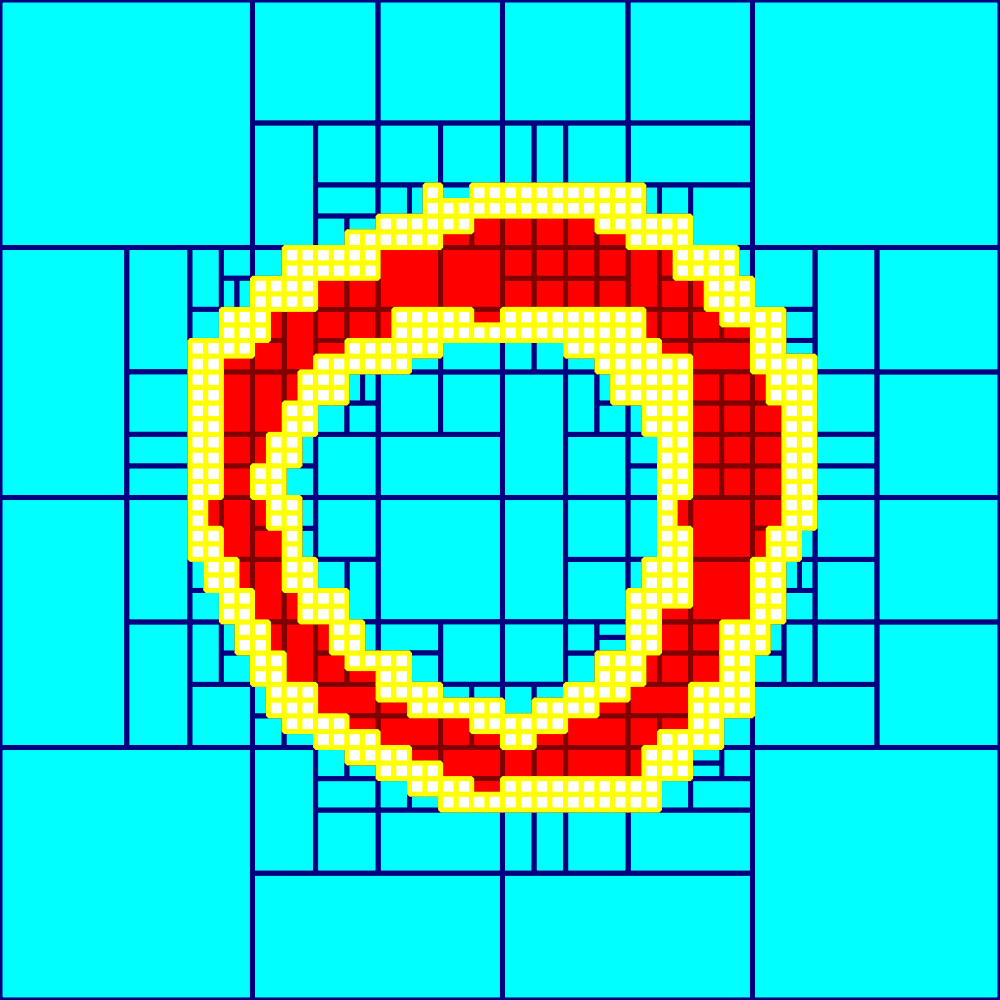
\includegraphics[scale=0.13]{subpaving1.png}
    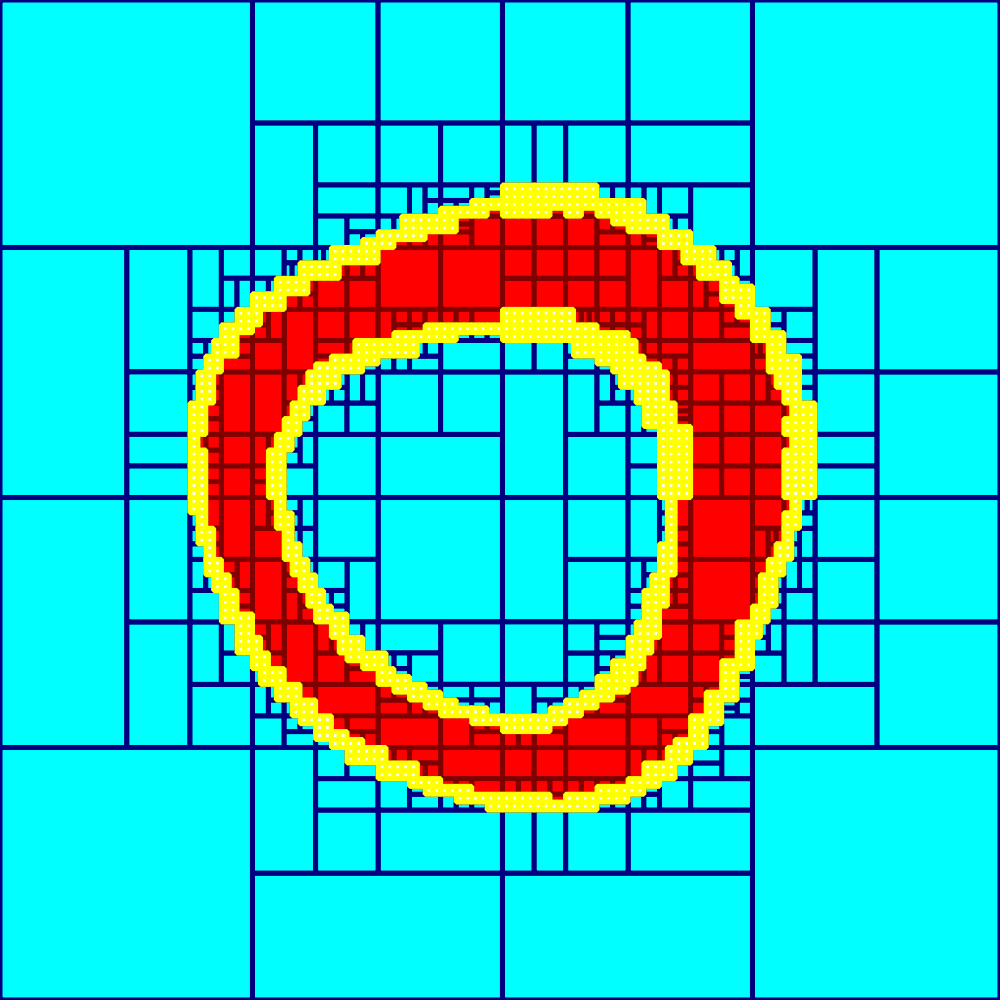
\includegraphics[scale=0.13]{subpaving2.png}
    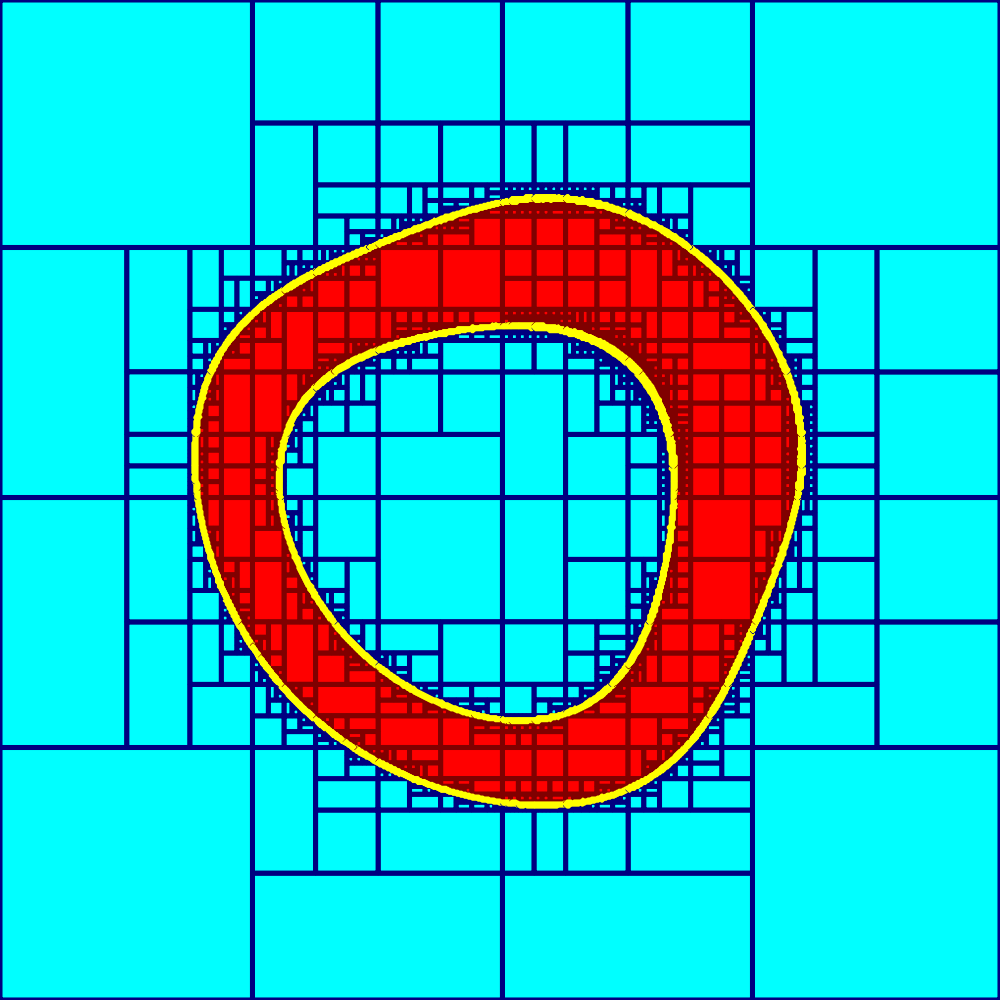
\includegraphics[scale=0.13]{subpaving3.png}
\end{frame}

\note{
    Traditionally we use decision trees to draw boxes/cells that would become inner (red) and outer (blue) approximations.
}

\begin{frame}
    \frametitle{Example: formulating problems with intervals}

    Problem 1:
    We have a power line with length between 60 to 70km.
    We want to be able to extend it to any length between 100 and 120km.
    What are the cable lengths should we should procure to make this possible? 
    Possible answer: $[30, 60]\km$

    \vspace{7mm}
    \par $(\forall a \in [60, 70]\km) (\forall t \in [100, 120]\km) (\exists x \in [30, 60]\km) (a + x = t)$

    \vspace{7mm}
    \par Letting $f(a, t) = t - a$, we say $[30, 60]\km$ is $(f, ([60, 70], [100, 120])\km^2)$-interpretable

\end{frame}

\note{
    In addition to the challenges posed by finding inner/outer approximations, doing mathematics with intervals involve extra logic. This is because we want to know whether statements about intervals apply to some elements in intervals, or only some numbers in intervals.

    Here if an interval is an answer to a formulation, we call it interpretable.
}

\begin{frame}
    \frametitle{Example: formulating problems with intervals}
    
    Problem 2:
    We have a power line with length between 60 to 70km. 
    We want to extend it to some arbitrary length between 100 and 120km.
    What cable lengths can we procure to make this possible?
    Possible answer: $[40, 50]\km$

    \vspace{7mm}
    \par $(\forall a \in [60, 70]\km) (\forall x \in [40, 50]\km) (\exists t \in [100, 120]\km) (a + x = t)$

    \vspace{7mm}
    \par Letting $f(a, t) = t - a$, we say $[50, 40]\km$ is $(f, ([60, 70], [120, 100])\km^2)$-interpretable.

\end{frame}

\note{
    Here we flip the intervals to express the predicates $\forall, \exists$ we use.
}

\begin{frame}
    \frametitle{Concepts: two desciptions of modal intervals}

    Description 1:
    \par Real interval set $\RIntervals$ contains intervals $[a, b], a \leq b$.
    \par Modal interval set $\Kaucher$ contains intervals $[a, b], a, b \in \Reals$

    \vspace{7mm}
    Description 2:
    \par A modal interval $A = (A', Q_A)$ is an element of the cartesian product $\RIntervals \times \set{\forall, \exists}$.
    \par Real interval set $\RIntervals \cong \RIntervals \times \set{\forall}$

\end{frame}

\note{
    Research in intervals have in the past been done by isolated groups, some which did not know about modal intervals, some which provided different descriptions of modal intervals.

    The first appearance was in $1980$ from E. Kaucher's paper \textit{Interval Analysis in the Extended Interval Space in IR} with the purpose of extending classical intervals to a metric space and lattice.

    Later, other in reachability research the second description was created to address the difference in formulating questions as seen in the example earlier.
}

\begin{frame}
    \frametitle{Concepts: two desciptions of modal intervals}

    \begin{columns}[T]
        \begin{column}{.5\textwidth}
            The two definitions are equivalent:

            \vspace{7mm}
            For $[a, b] \in \Kaucher$,
            \par $[a, b] = \begin{cases}
                ([a, b]', \exists) \text{ if } a \leq b \; \text{(proper)} \\
                ([b, a]', \forall) \text{ if } a > b \; \text{(improper)} \\
                            \end{cases}$

            \vspace{7mm}
            For real numbers $[a, a]$, $\forall, \exists$ quantifies are interchangable.

        \end{column}
        \begin{column}{.5\textwidth}
            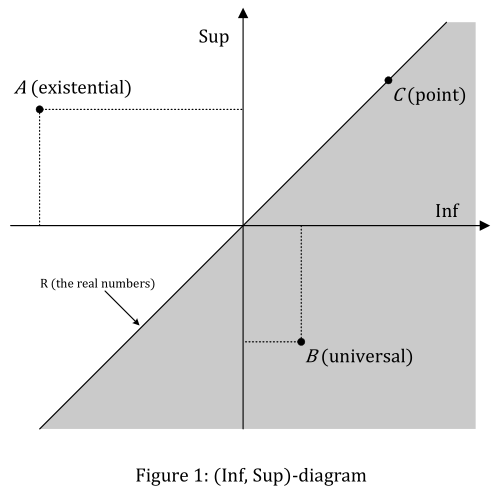
\includegraphics[scale=0.3]{inf-sup-diagram.png}

        \end{column}
    \end{columns}

\end{frame}

\note{
    The intervals with a mark on them are classical intervals i.e. $A', [a, b]'$ are classical intervals.
}

\begin{frame}
    \frametitle{Operations}

    \begin{columns}[T]
        \begin{column}{.5\textwidth}
            $\Sup([a, b]) = b$
            \par $\Inf([a, b]) = a$
            \par $\dual([a, b]) = [b, a]$
            \par $\wid([a, b]) = b - a$

            \vspace{7mm}
            \par metric: $d([a_1, b_1], [a_2, b_2]) = \max(|a_1 - a_2|, |b_1 - b_2|)$

            \vspace{7mm}
            $\prop([a, b]) = [\min(a, b), \max(a, b)]$
            
            \vspace{7mm}
            \par We denote interval variables $[x] = [a, b]$

        \end{column}
        \begin{column}{.5\textwidth}
            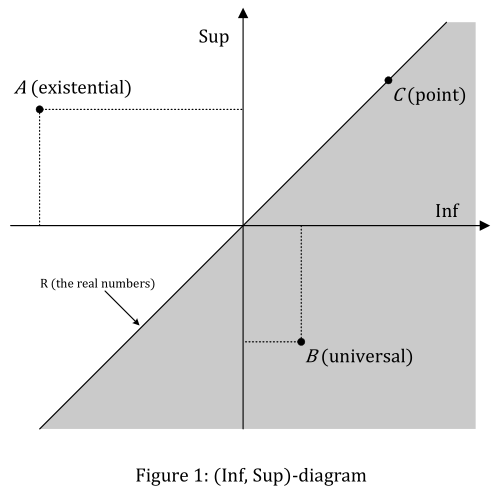
\includegraphics[scale=0.3]{inf-sup-diagram.png}

        \end{column}
    \end{columns}

\end{frame}

\note{
    wid does not take the absolute of $b - a$ so improper intervals will have negative width. We will use some of these operations later.
}

\begin{frame}
    \frametitle{Definition: k-dimensional modal intervals}

    k-dimensional modal intervals $[\bm{x}] = ([x_1], \ldots, [x_k]) \in \Kaucher^k$

    \vspace{7mm}
    Modal interval matrixes are defined similarly.

    \vspace{7mm}
    We can partition interval arrays into proper-improper components $[\bm{x}] = ([\bm{x}_\cP], [\bm{x}_\cI])$ where
    $\cP = \set{k : [x_k] \in \RIntervals}$ and $\cI = \set{k : [x_k] \not\in \RIntervals}$.

\end{frame}

\note{
    Not shown are interval matrices that are just matrices with interval elements.
}

\begin{frame}
    \frametitle{Definition: $(f,[\bm{x}])$-interpretability}
 
    Given a continuous function $f: \Reals^n \ra \Reals$ and $[\bm{x}] \in \Kaucher^n$ we want to compute $[z] \in \Kaucher$ such that the following quantified proposition is true:

    \vspace{7mm}
    $(\forall \bm{x}_\cP \in [\bm{x}_\cP]) (Q_z z \in [z]) (\exists \bm{x}_\cI \in [\bm{x}_\cI]) (f(\bm{x}) = z)$

    \vspace{7mm}
    where $\cP = \set{k : [x_k] \in \RIntervals}$, $\cI = \set{k : [x_k] \not\in \RIntervals}$ and $Q_z = \exists$ if $[z] \in \RIntervals$, $Q_z = \forall$ otherwise.

    \vspace{7mm}
    We call $[z]$ an interval that is $(f,[\bm{x}])$-interpretable.
\end{frame}

\note{
    The rest of this presentation (and all the research revolving intervals such as software verification / reachability) revolves this one definition. This is the general version of the example with power lines we saw earlier. This is how we formulate problems using intervals. You can say this is an extension of equality in algebra.
}

\begin{frame}
    \frametitle{Example: $(f,[\bm{x}])$-interpretability}
 
    Given a continuous function $f: \Reals^n \ra \Reals$, $[\bm{x}] \in \Kaucher^n$, $[z] \in \Kaucher$:

    \vspace{7mm}
    If $[\bm{x}] \in \RIntervals^n$ and $[z] \in \RIntervals$ then 
    $(\exists z \in [z]) (\forall \bm{x} \in [\bm{x}]) (f(\bm{x}) = z)$ \par
    so $[z]$ is an outer approximation


    \vspace{7mm}
    If $[\bm{x}] \not\in \RIntervals^n$ and $[z] \not\in \RIntervals$ then 
    $(\forall z \in [z]) (\exists \bm{x} \in [\bm{x}]) (f(\bm{x}) = z)$ \par
    making $[z]$ an inner approximation

\end{frame}

\note{
    In verification research we use these particular instances of the general quantified proposition.
}

\begin{frame}
    \frametitle{Definition: subsets - comparing $(f,[\bm{x}])$-interpretable intervals}
 
    Given a continuous function $f: \Reals^n \ra \Reals$, $[\bm{x}] \in \Kaucher^n$, $[z], [z'] \in \Kaucher$ are intervals that are $(f,[\bm{x}])$-interpretable.

    \vspace{2mm}
    If $[z'] \subseteq [z]$ then $[z']$ is more accurate than $[z]$

    \vspace{7mm}
    $A \subseteq B \; \equiv \begin{cases}
        A' \subseteq B' \; \text{ if } A, B \in \RIntervals \\
        A' \supseteq B' \; \text{ if } A, B \not\in \RIntervals \\
        A' \cap B' \neq \varnothing \; \text{ if } A \not\in\RIntervals, B \in\RIntervals \\
        A' = B' = [a, a]' \; \text{ if } A \in\RIntervals, B \not\in\RIntervals \\
    \end{cases}$

\end{frame}

\note{
    A problem involving intervals can have more than one solution. We can compare solutions by extendeing subsets to modal intervals.

    Extending subset comparisons allows us to generalize the rounding process in verification /reachability: outer roundings for proper intervals and inner roundings for improper intervals
}

\begin{frame}
    \frametitle{Question: AE-extensions}
 
    We call $[z]$ an interval that is $(f,[\bm{x}])$-interpretable... but how do we reliably obtain $[z]$?

    \vspace{7mm}
    Given a continuous function $f: \Reals^n \ra \Reals$, we wish to obtain an AE-extension, that is a function $f: \Kaucher^n \ra \Kaucher$ such that $\forall [\bm{x}] \in \Kaucher^n, f([\bm{x}])$ is $(f, [\bm{x}])$-interpretable.

\end{frame}

\note{
    An open problem is the question of producing AE-extensions. Here I've decided to abuse the letter $f$ to mean both the original function and an AE-extension. Which one I am using depends on what kind of variables are passed in.
}

\begin{frame}
    \frametitle{Question: AE-extensions}
 
    We call $[z]$ an interval that is $(f,[\bm{x}])$-interpretable... but how do we reliably obtain $[z]$?

    \vspace{7mm}
    Given a continuous function $f: \Reals^n \ra \Reals$, we wish to obtain an AE-extension, that is a function $f: \Kaucher^n \ra \Kaucher$ such that $\forall [\bm{x}] \in \Kaucher^n, f([\bm{x}])$ is $(f, [\bm{x}])$-interpretable.

    \vspace{7mm}
    Can we construct $f$ from \textit{elementary functions}?

\end{frame}

\begin{frame}
    \frametitle{Extending elementary functions}

    Addition: $[a_1, a_2] + [b_1, b_2] = [a_1 + b_1, a_2 + b_2]$ \par
    Subtraction: $[a_1, a_2] - [b_1, b_2] = [b_1 - a_1, b_2 - a_2]$
    \vspace{7mm}

    \begin{columns}[T]
        \begin{column}{.5\textwidth}
            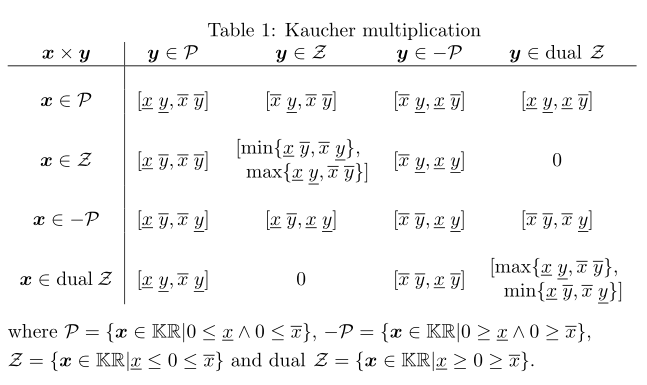
\includegraphics[scale=0.3]{kaucher-mult.png}

        \end{column}
        \begin{column}{.5\textwidth}
            \begin{center}
                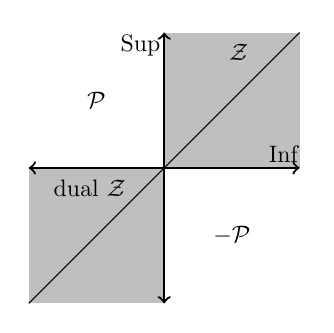
\begin{tikzpicture}[thick,scale=0.86, every node/.style={transform shape}]
                    \fill[lightgray] (0,0) rectangle (2,2);
                    \fill[lightgray] (2,2) rectangle (4,4);
                    \draw [<->] (0,2) -- (4,2);
                    \draw [<->] (2,0) -- (2,4);
                    \draw [thin, -] (4,4) -- (0,0);
                    \node at (1,3) {$\cP$};
                    \node at (3,1) {$-\cP$};
                    \node at (3.76, 2.2) {Inf};
                    \node at (1.65, 3.8) {Sup};
                    \node at (0.9,1.7) {dual $\mathcal{Z}$};
                    \node at (3.1,3.7) {$\mathcal{Z}$};
                \end{tikzpicture}
            \end{center}
        \end{column}
    \end{columns}

\end{frame}

\begin{frame}
    \frametitle{Properties of elementary functions}

    Additive identity : $[a_1, a_2] + [0, 0] = [a_1, a_2] = [0, 0] + [a_1, a_2]$
    \par Additive inverse: $[a_1, a_2] + -\dual([a_1, a_2]) = [a_1, a_2] + [-a_1, -a_2] = [0, 0]$

    \vspace{7mm}
    Multiplicative identity: $[a_1, a_2] * [1, 1] = [a_1, a_2] = [1, 1] * [a_1, a_2]$
    \par Multiplicative inverse: if $0 \not\in \prop([a_1, a_2])$ then $[a_1, a_2] * \frac{1}{\dual([a_1, a_2])} = [a_1, a_2] * \arr{\frac{1}{a_2}, \frac{1}{a_1}} = [1, 1]$


    \vspace{7mm}
    $(\Kaucher, +, \times)$ is \textit{not} a Ring \par
    $A(B + C) \subseteq AB + AC$ if $A$ is proper, and $A(B + C) \supseteq AB + AC$ if $A$ is improper.
\end{frame}

\begin{frame}
    \frametitle{Theorem: JM-commutivity}

    Every one variable continuous function $f: \Reals \ra \Reals$ is JM-commutable: for $A \in \Kaucher$ \par
    \vspace{2mm}
    $f(A) = \begin{cases}
        [\min_{x \in A} f(x), \max_{x \in A} f(x)] \quad \text{ if } A \text{ is proper} \\
        [\max_{x \in A} f(x), \min_{x \in A} f(x)] \quad \text{ if } A \text{ is improper} \\
    \end{cases}$

    \vspace{7mm}
    Examples:
    \vspace{2mm}
    $sin(A) = \begin{cases}
        [\min_{x \in A} sin(x), \max_{x \in A} sin(x)] \quad \text{ if } A \text{ is proper} \\
        [\max_{x \in A} sin(x), \min_{x \in A} sin(x)] \quad \text{ if } A \text{ is improper} \\
    \end{cases}$

\end{frame}

\note{
    There's actually much literature revolving JM-commutivity using lattice operations. Here is one of the main results that I will not prove. This is convenient because it allows us to extend every single value function.
}

\begin{frame}
    \frametitle{Example: JM-commutivity}

    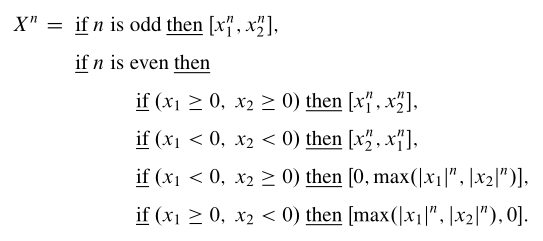
\includegraphics[scale=0.4]{kaucher-pow.png}

    \vspace{7mm}
    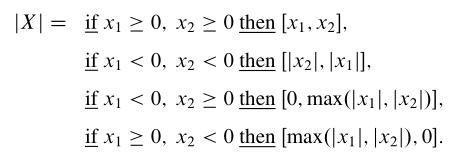
\includegraphics[scale=0.4]{kaucher-abs.png}

\end{frame}

\begin{frame}
    \frametitle{AE-extensions: general interval extension vs. mean value extension}

    Let $f: \Reals^n \ra \Reals$, $[\bm{x}] \in \Kaucher^n$

    \vspace{7mm}
    General interval extension: \par
    If $f(x_1, \ldots, x_n)$ can be expressed in elementary functions where each variable appears only once, then $f([\bm{x}])$ calculated by replacing each $x_i$ by $[x_i]$ is $(f,[\bm{x}])$-interpretable.

    \vspace{7mm}
    Mean value extension: \par
    Let $\bm{\Delta} \in \RIntervals^n$ such that $\set{\frac{\partial f}{\partial x_i}(x) : x \in \prop([\bm{x}])} \subseteq \Delta_i$. \par
    Then $\fMV([\bm{x}]) := f(\tilde{x}) + \bm{\Delta} \cdot ([\bm{x}] - \tilde{x})$ is $(f, [\bm{x}])$-interpretable for all $\tilde{x} \in \prop([\bm{x}])$.

    \vspace{7mm}
    ($\Delta$ can be interval approx. of a gradient or Jacobian)
\end{frame}

\note{
    The mean value extension implicitly uses the general interval extension because we are extending the function $\fMV(\bm{x}) := f(\tilde{x}) + \bm{\delta}(\bm{x} - \tilde{x})$ which is guaranteed to give us $(\fMV,[\bm{x}])$-interpretability

    The formula uses dot product. Both dot product and matrix-vector multiplication utilize the elementary binary operations we extended earlier. Here we are free to choose $\Delta$ and $\tilde{x}$, but we usually choose the gradient. 
    
    Note this mean-value extension is not limited to vector-scalar functions. For vector-vector functions we replace $\Delta$ with a matrix. I'll show you an example in the second part.
}

\begin{frame}
    \frametitle{Order of convergence for AE-extensions}

    How do these two kinds of extensions compare?

    \vspace{7mm}
    Definition: order of convergence $\alpha$ \par
    The AE-extension for $f$ has an order of convergence $\alpha \in \Reals, \alpha > 0$ if and only if there exists a minimal AE-extension $h: \RIntervals^n \ra \RIntervals$ for $f$ such that $\forall [\bm{y}] \in \RIntervals^n, \exists \gamma > 0, \forall [x] \in \bm{K}[\bm{y}]$ we have

    \vspace{2mm}
    $|| \wid(h([\bm{x}])) - \wid(f([\bm{x}])) || \leq \gamma || \wid([\bm{x}]) || ^\alpha$

    \vspace{7mm}
    \begin{enumerate}
        \item General interval extension: linear order ($\alpha = 1$)
        \item Mean value extension: quadratic order ($\alpha = 2$)
        \item a minimal AE-extension $h$ of $f$ always exists, but may not be feasible.
        \item $\bm{K}[\bm{y}] = \set{[a, b] : a, b \in [\bm{y}]}$
    \end{enumerate}

\end{frame}

\note{
    The existance of a minimal AE-extension for every continuous real function on $\Reals^n$ is will always exist by a proposition in A. Goldsztejn's work. Given a interval box, consider the range $f$ with the box, the minimal AE-extension $h$ is the one that produces the tightest possible box around the range.
$|| \cdot ||$ is the canonical distance norm in $\Reals^n$
From the result, mean-value extensions are a lot better.
}

\begin{frame}
    \frametitle{Part 2: Inner Approximated Reachability Analysis}

    Covering:


    \vspace{2mm}
    \sout{Eric Goubault, Olivier Mullier and Sylvie Putot (French Alternative Energies and Atomic Energy Commission (CEA)), Michel Kieffer (French National Center for Scientific Research (CNRS))
    \textit{Inner Approximated Reachability Analysis} (HSCC 2014)}

    \vspace{2mm}
    Eric Goubault and Sylvie Putot (French Alternative Energies and Atomic Energy Commission (CEA))
    \textit{Forward Inner-Approximated Reachability of Non-Linear Continuous Systems} (HSCC 2017)
\end{frame}

\note{
This is a last minute change. I just realized it is not appropriate for me to do the HSCC 2014 paper since it does not immediately follow from part 1. That said it this one we're doing is less complicated.

French National Center for Scientific Research (CNRS)
A budget of 3.3 billion euros,
33,000 people dedicated to research,
1,144 research laboratories in France and abroad

Goubault - verification of numerical programs and systems, on geometric methods for concurrency, directed topology and applications to verification of concurrent, distributed and fault-tolerant computing
Putot - verification of numerical programs and systems; present work focuses on the verification of hybrid, or more generally Cyber-Physical Systems
}

\newcommand{\intervalbox}[1]{\arr{\bm{x}^{(#1)}}}
\newcommand{\tintervalbox}[1]{\arr{\tilde{\bm{x}}^{(#1)}}}
\newcommand{\enclosure}[1]{\arr{\bm{r}^{(#1)}}}
\newcommand{\tenclosure}[1]{\arr{\tilde{\bm{r}}^{(#1)}}}
\newcommand{\autof}[1]{\bm{f}^{[#1]}}

\begin{frame}
    \frametitle{Problem}
    
    Problem specification:
    an autonomous ODE $\dot{\bm{x}} = \bm{f}(\bm{x})$ where $\bm{f}: \Reals^n \ra \Reals^n$ is infinitely differentiable, a time interval $[0,\tau]$ and initial conditions $\intervalbox{0} \in \RIntervals$

    \vspace{7mm}
    Goal:
    Find tight inner approximation of reachable states for all initial conditions in $\intervalbox{0}$ over time interval.
\end{frame}

\note{
    This problem appeared in both the HSCC 2014 and 2017 papers. We have almost all the tools from part 1 to solve this problem so I've simplified this part to showing how the algorithm itself and how it implements interpretability for inner/outer approximtions.
}

\begin{frame}
    \frametitle{Solution}

    Given partitions $[t_j, t_{j+1}]$ of $[0, \tau]$...
 
    \vspace{7mm}
    Use automatic differentiation to obtain the coefficients of the $k$-th order taylor approximation for $\bm{x}(t)$:

    \begin{enumerate}
        \item $\autof{1} = \bm{f}$

        \vspace{2mm}
        \item $\autof{i+1} = J(\autof{i}) \cdot \bm{f}$

        \vspace{2mm}
        \item Aproximate $\enclosure{j+1}$

        \vspace{2mm}
        \item For $t \in [t_j, t_{j+1}]$, $\bm{x}(t, t_j, \intervalbox{j}) = \intervalbox{j} + \sum^{k-1}_{i=0} (t - t_j)^i \frac{\autof{i}(\intervalbox{j})}{i!} + (t - t_j)^k \frac{\autof{k}(\enclosure{j+1})}{k!}$

        \vspace{2mm}
        \item $\intervalbox{j+1} = \bm{x}(t_{j+1}, t_j, \intervalbox{j})$
    \end{enumerate}
    
\end{frame}

\note{
    We are using taylor models with enclosures for tail approximation of the taylor series.
}

\begin{frame}
    \frametitle{Solution}

    Starting from a point $\tilde{x}^{(0)} \in \intervalbox{0}$ initialize $\tintervalbox{0} = \tilde{x}^{(0)}$

    \begin{enumerate}
        \item Aproximate $\tenclosure{j+1}$

        \vspace{2mm}
        \item For $t \in [t_j, t_{j+1}]$, $\tilde{\bm{x}}(t, t_j, \tintervalbox{j}) = \tintervalbox{j} + \sum^{k-1}_{i=0} (t - t_j)^i \frac{\autof{i}(\tintervalbox{j})}{i!} + (t - t_j)^k \frac{\autof{k}(\tenclosure{j+1})}{k!}$

        \vspace{2mm}
        \item $\tintervalbox{j+1} = \tilde{\bm{x}}(t_{j+1}, t_j, \tintervalbox{j})$
    \end{enumerate}
    
\end{frame}

\newcommand{\Jac}{\text{Jac}_{\bm{x}}}
\newcommand{\Enclosure}[1]{\arr{\bm{R}^{(#1)}}}
\newcommand{\Intervalbox}[1]{\arr{\bm{J}^{(#1)}}}

\begin{frame}
    \frametitle{Solution}

    Obtain taylor approximation of the Jacobian of $\bm{x}(t)$. Let \par
    \[\Jac f = \bmat
    \frac{\partial f_1}{\partial x_1} & \cdots & \frac{\partial f_1}{\partial x_n} \\
    \vdots & & \vdots \\
    \frac{\partial f_n}{\partial x_1} & \cdots & \frac{\partial f_n}{\partial x_n}
    \emat\]

    \vspace{7mm}
    \begin{enumerate}
        \item Aproximate $\Enclosure{j+1}$

        \vspace{2mm}
    \item For $t \in [t_j, t_{j+1}]$, $\bm{J}(t, t_j, \intervalbox{j}) = \Intervalbox{j} + \sum^{k-1}_{i=0} (t - t_j)^i \frac{\Jac\autof{i}(\Intervalbox{j})}{i!} \cdot \Intervalbox{j} + (t - t_j)^k \frac{\Jac\autof{k}(\enclosure{j+1})}{k!} \cdot \Enclosure{j+1}$

        \vspace{2mm}
        \item $\Intervalbox{j+1} = \bm{J}(t_{j+1}, t_j, \intervalbox{j})$
    \end{enumerate}
    
\end{frame}

\begin{frame}
    \frametitle{Solution}
    
    Recall mean-value AE-extension: \par
    Let $f: \Reals^n \ra \Reals$, $[\bm{x}] \in \Kaucher^n$ \par
    and $\bm{\Delta} \in \RIntervals^n$ such that $\set{\frac{\partial f}{\partial x_i}(x) : x \in \prop([\bm{x}])} \subseteq \Delta_i$. \par
    Then $\fMV([\bm{x}]) := f(\tilde{x}) + \bm{\Delta}([\bm{x}] - \tilde{x})$ is $(f, [\bm{x}])$-interpretable for all $\tilde{x} \in \prop([\bm{x}])$.
 
    \vspace{7mm}
    Define: \par
    $]\bm{x}[(t, t_j) := \tilde{\bm{x}}(t, t_j, \tintervalbox{j}) + \bm{J}(t, t_j, \intervalbox{j})(\dual\intervalbox{0} - \tilde{\bm{x}}^{(0)})$

    \vspace{2mm}
    If it is improper for given $t$, then $]\bm{x}[(t, t_j)$ is an inner approximation.
\end{frame}

\note{
    From the values we got in the last 3 slides we combine it to create a function that computes the inner approximation. Here we assume $\intervalbox{0}$ is proper and its dual is the interval with endpoints flipped. Sometimes the inner approximation is empty however.
}

\begin{frame}
    \frametitle{Solution: Vanderpoll}

    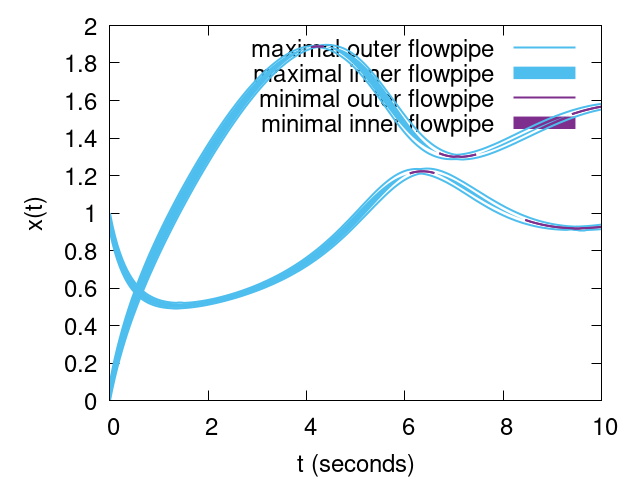
\includegraphics[scale=0.4]{xi.png}
    
\end{frame}

\end{document}
